\documentclass[11pt]{report}

\usepackage[T1]{fontenc}
\usepackage[utf8]{inputenc}
\usepackage{lmodern}
\usepackage{microtype}
\usepackage[a4paper,margin=0.9in]{geometry}
\usepackage{xcolor}
\usepackage{graphicx}
\usepackage{booktabs}
\usepackage{tabularx}
\usepackage{longtable}
\usepackage{array}
\usepackage{enumitem}
\usepackage{setspace}
\usepackage{titlesec}
\usepackage{fancyhdr}
\usepackage{lastpage}
\usepackage{float}
\usepackage{hyperref}
\usepackage{xurl}
\usepackage{listings}
\usepackage[most]{tcolorbox}
\usepackage{tikz}
\usetikzlibrary{arrows.meta,positioning,fit,calc,shapes.geometric}

\definecolor{navy}{HTML}{153A5B}
\definecolor{teal}{HTML}{1F6F78}
\definecolor{gold}{HTML}{C79A3B}
\definecolor{slate}{HTML}{425466}
\definecolor{mist}{HTML}{F4F7FA}
\definecolor{softline}{HTML}{D9E2EC}
\definecolor{ink}{HTML}{1E293B}
\definecolor{success}{HTML}{0F766E}
\definecolor{warning}{HTML}{B45309}
\definecolor{danger}{HTML}{B91C1C}

\hypersetup{
  colorlinks=true,
  linkcolor=navy,
  urlcolor=teal,
  citecolor=navy,
  pdftitle={TRP Week 7 Technical Report},
  pdfauthor={Birkity Yishak}
}

\setstretch{1.08}
\setlength{\parindent}{0pt}
\setlength{\parskip}{0.5em}

\titleformat{\chapter}[display]
  {\normalfont\bfseries\color{navy}}
  {\filleft\Large\chaptername\ \thechapter}
  {0.3em}
  {\titlerule[1pt]\vspace{0.8ex}\Huge}
  [\vspace{0.4ex}\titlerule]

\titleformat{\section}
  {\normalfont\Large\bfseries\color{teal}}
  {\thesection}
  {0.6em}
  {}

\titleformat{\subsection}
  {\normalfont\large\bfseries\color{navy}}
  {\thesubsection}
  {0.6em}
  {}

\pagestyle{fancy}
\fancyhf{}
\fancyhead[L]{\textcolor{navy}{TRP Week 7 Technical Report}}
\fancyhead[R]{\textcolor{slate}{Birkity Yishak}}
\fancyfoot[L]{\textcolor{slate}{Data Contract Enforcer}}
\fancyfoot[R]{\textcolor{slate}{Page \thepage\ of \pageref{LastPage}}}
\renewcommand{\headrulewidth}{0.4pt}
\renewcommand{\footrulewidth}{0.4pt}

\lstdefinestyle{codestyle}{
  basicstyle=\ttfamily\small,
  backgroundcolor=\color{mist},
  frame=single,
  rulecolor=\color{softline},
  breaklines=true,
  columns=fullflexible,
  keepspaces=true
}

\newtcolorbox{callout}[1][]{
  enhanced,
  colback=mist,
  colframe=navy,
  arc=2mm,
  boxrule=0.8pt,
  left=2mm,
  right=2mm,
  top=1.5mm,
  bottom=1.5mm,
  #1
}

\newtcolorbox{statusbox}[2][]{
  enhanced,
  colback=#2!8,
  colframe=#2!75!black,
  arc=2mm,
  boxrule=0.8pt,
  left=2mm,
  right=2mm,
  top=1.5mm,
  bottom=1.5mm,
  #1
}

\newcolumntype{L}[1]{>{\raggedright\arraybackslash}p{#1}}
\newcolumntype{Y}{>{\raggedright\arraybackslash}X}
\newcommand{\codecell}[1]{{\small\path{#1}}}

\begin{document}

\begin{titlepage}
\pagecolor{mist}
\centering
\vspace*{1.7cm}

{\Huge\bfseries\color{navy} TRP Week 7 Technical Report\par}
\vspace{0.5cm}
{\Large\color{teal} Data Contract Enforcer -- Implementation Through Phase 3\par}
\vspace{1.2cm}

\begin{tcolorbox}[width=0.9\textwidth,colback=white,colframe=navy,boxrule=1pt,arc=2mm]
\centering
{\Large\bfseries Candidate: Birkity Yishak\par}
\vspace{0.3cm}
{\large Challenge: Week 7 Data Contract Enforcer\par}
\vspace{0.2cm}
{\large Date: April 1, 2026\par}
\vspace{0.2cm}
{\large Repository: \texttt{data-contract-enforcer}\par}
\end{tcolorbox}

\vfill

\begin{tcolorbox}[width=0.88\textwidth,colback=white,colframe=teal,boxrule=0.8pt,arc=2mm]
\raggedright
\textbf{Implementation scope covered in this report}
\begin{itemize}[leftmargin=1.5em,itemsep=0.3em]
  \item Phase 0: domain analysis, canonical schema gap analysis, and upstream system readiness.
  \item Phase 1: ContractGenerator for Week 3 extractions using real JSONL data and lineage context.
  \item Phase 2: ValidationRunner with structural and statistical checks plus injected violation detection.
  \item Phase 3: ViolationAttributor with git-backed blame chain generation and blast-radius reasoning.
\end{itemize}
\end{tcolorbox}

\vfill
{\large\color{slate} 10 Academy -- Transitional Research Program\par}
\vspace{0.5cm}
{\small\color{slate} This document is written as an engineering report for the current implementation state.\par}

\end{titlepage}
\nopagecolor

\tableofcontents
\clearpage

\chapter*{Executive Overview}
\addcontentsline{toc}{chapter}{Executive Overview}

\begin{statusbox}{success}
\textbf{Implementation verdict:} the system is operational through Phase 3.
The repository can now generate a real contract from Week 3 data, validate that contract against clean and violated snapshots, and attribute the resulting failure back to a plausible producer-side file and commit in the Week 3 source repository.
\end{statusbox}

\section*{Why this checkpoint matters}
The Week 7 challenge is not only about writing validation code. It is about demonstrating that upstream systems can be turned into contract-aware interfaces, that silent failures can be detected with evidence, and that the engineering team can move from ``something broke'' to ``here is the most likely place it broke and what might be affected.'' This checkpoint is therefore already meaningful if it proves three things:

\begin{itemize}[leftmargin=1.5em]
  \item The contract is grounded in \textbf{real system outputs}, not a fabricated toy schema.
  \item The validator catches both \textbf{hard structural problems} and \textbf{semantic drift}.
  \item Attribution produces a \textbf{defensible triage path}, even if downstream blast radius is still partial.
\end{itemize}

\section*{Outcome in one paragraph}
This implementation satisfies those three conditions. Week 3 data was migrated into the canonical extraction shape expected by Week 7. A profiling-based ContractGenerator builds a readable YAML contract from the actual fields and distributions present in that dataset. A ValidationRunner then validates the dataset, stores numeric baselines, and correctly fails when fact-level confidence values are scaled from \texttt{0.0--1.0} to \texttt{0--100}. Finally, a ViolationAttributor traces the failure back to the Week 3 Document Intelligence Refinery repository, ranking the producer-side files that define and persist confidence behavior. The main remaining technical weakness is not validation logic; it is that the current Week 4 lineage snapshots still do not expose an explicit Week 3 consumer path, which limits downstream blast-radius enrichment.

\clearpage
\chapter{Challenge Framing and Project Objectives}

\section{Problem statement}
The Data Contract Enforcer exists to answer two questions that appear in production systems constantly:

\begin{enumerate}[leftmargin=1.6em]
  \item Can we stop a producer system from breaking downstream consumers silently?
  \item If a break happens anyway, can we detect it quickly and trace it back to a responsible change?
\end{enumerate}

In this repository, those questions are tested against outputs inherited from Weeks 1 through 5. The most important early interface for the current implementation is Week 3, because its extraction payload contains a naturally risky field: confidence. Confidence values are numerically typed, which means type checks alone are insufficient. A \texttt{0.0--1.0} field can quietly become \texttt{0--100} and still remain ``numeric.'' That is exactly the kind of failure that creates incidents in real data systems.

\section{Current scope}
This report covers implementation through Phase 3:

\begin{itemize}[leftmargin=1.5em]
  \item \textbf{Phase 0} -- evidence-based domain notes, schema-gap analysis, and real output inspection.
  \item \textbf{Phase 1} -- contract generation from actual Week 3 extractions, including field profiling and lineage notes.
  \item \textbf{Phase 2} -- validation on clean and violated data, with baseline creation and statistical drift checks.
  \item \textbf{Phase 3} -- failure normalization, git-backed blame-chain generation, and blast-radius reasoning.
\end{itemize}

\section{What this report intentionally does not claim}
This report does not claim that the full Week 7 system is complete. The following remain out of scope at this checkpoint:

\begin{itemize}[leftmargin=1.5em]
  \item SchemaEvolutionAnalyzer
  \item AI Contract Extensions
  \item the final auto-generated Enforcer Report
  \item a fully canonical Week 4 lineage snapshot with explicit Week 3 downstream consumers
\end{itemize}

\begin{callout}
\textbf{Success criterion:} if a reviewer can inspect this repository and verify that contract generation, validation, and attribution all run on real Week 3 data with reproducible outputs, then the current implementation has achieved its purpose.
\end{callout}

\clearpage
\chapter{Upstream Data and Canonicalization}

\section{Source systems used}
The repository brings together outputs from prior weekly systems. The current build focuses on the interfaces that matter most for contract enforcement, while still acknowledging the broader upstream landscape.

\begin{center}
\small
\setlength{\tabcolsep}{4pt}
\renewcommand{\arraystretch}{1.25}
\begin{tabularx}{\textwidth}{L{1.05in} L{1.7in} Y L{0.95in}}
\toprule
System & File & Current role & Status \\
\midrule
Week 1 & \codecell{outputs/week1/intent_records.jsonl} & evidence for schema variety and Phase 0 domain notes & present \\
Week 2 & \codecell{outputs/week2/verdicts.jsonl} & evidence for verdict-envelope shape and future extensions & present \\
Week 3 & \codecell{outputs/week3/extractions.jsonl} & primary monitored interface for Phases 1--3 & canonicalized \\
Week 4 & \codecell{outputs/week4/lineage_snapshots.jsonl} & required lineage dependency for attribution and blast radius & canonical JSONL, enrichment still partial \\
Week 5 & \codecell{outputs/week5/events.jsonl} & event-stream source for later contract expansion & migrated envelope \\
Traces & \codecell{outputs/traces/runs.jsonl} & LangSmith trace evidence for later AI extensions & present \\
\bottomrule
\end{tabularx}
\end{center}

\section{Data flow diagram accuracy and schema annotation}
This report now makes the cross-system data map explicit rather than leaving it implied. The diagram below is intentionally conservative: it shows only flows that are actually represented by artifacts present in this repository. Where the underlying Week 4 lineage snapshots still lack an explicit Week 3 consumer path, that limitation is stated in the annotation rather than hidden.

\begin{figure}[H]
\centering
\resizebox{\textwidth}{!}{
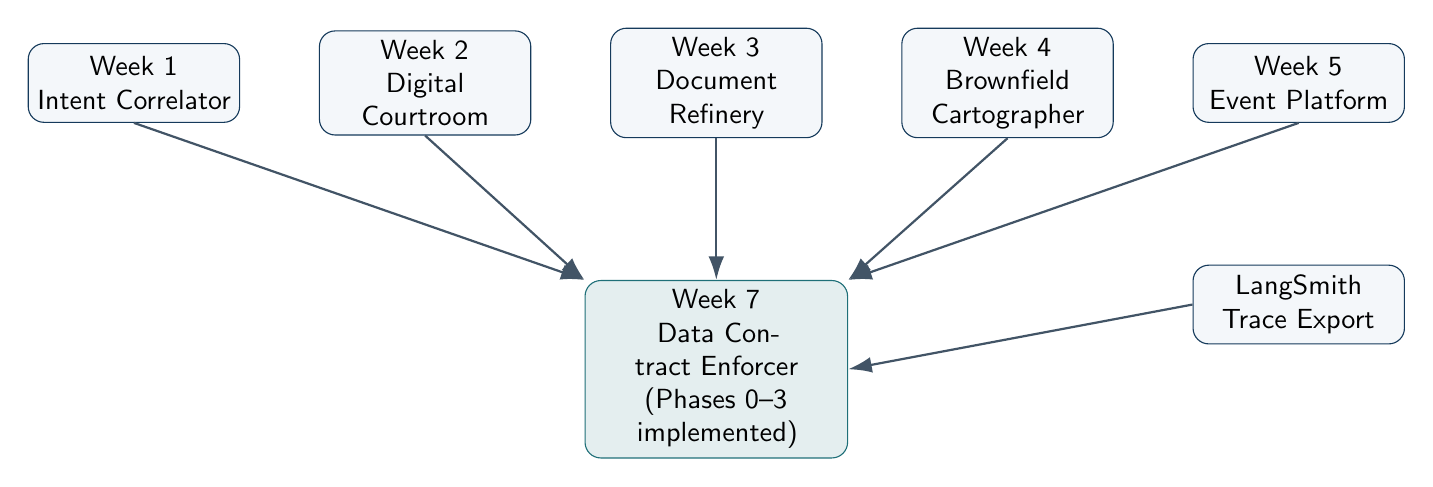
\begin{tikzpicture}[
  font=\sffamily,
  node distance=0.9cm and 1.0cm,
  sys/.style={draw=navy, rounded corners=2mm, fill=mist, minimum width=2.45cm, minimum height=1.0cm, align=center, text width=2.45cm},
  core/.style={draw=teal, rounded corners=2mm, fill=teal!12, minimum width=3.1cm, minimum height=1.2cm, align=center, text width=3.1cm},
  arrow/.style={-{Latex[length=3mm,width=2mm]}, thick, draw=slate}
]
  \node[sys] (w1) {Week 1\\Intent Correlator};
  \node[sys, right=of w1] (w2) {Week 2\\Digital Courtroom};
  \node[sys, right=of w2] (w3) {Week 3\\Document Refinery};
  \node[sys, right=of w3] (w4) {Week 4\\Brownfield Cartographer};
  \node[sys, right=of w4] (w5) {Week 5\\Event Platform};

  \node[core, below=1.8cm of w3] (enforcer) {Week 7\\Data Contract Enforcer\\(Phases 0--3 implemented)};
  \node[sys, below=1.8cm of w5] (ls) {LangSmith\\Trace Export};

  \draw[arrow] (w1.south) -- (enforcer.north west);
  \draw[arrow] (w2.south) -- (enforcer.north west);
  \draw[arrow] (w3.south) -- (enforcer.north);
  \draw[arrow] (w4.south) -- (enforcer.north east);
  \draw[arrow] (w5.south) -- (enforcer.north east);
  \draw[arrow] (ls.west) -- (enforcer.east);
\end{tikzpicture}
}
\caption{Inter-system data flow used for this implementation.}
\end{figure}

The diagram is accurate in the sense that each arrow corresponds to a concrete artifact, and each artifact has a schema annotation that can be checked against the repository.

\begin{center}
\small
\setlength{\tabcolsep}{4pt}
\renewcommand{\arraystretch}{1.2}
\begin{tabularx}{\textwidth}{L{1.1in} L{1.55in} Y L{0.95in}}
\toprule
Flow & Artifact & Schema annotation used in this report & Accuracy note \\
\midrule
Week 1 $\rightarrow$ Week 7 & \codecell{intent_records.jsonl} & \texttt{intent\_id}, \texttt{description}, \texttt{code\_refs[]}, \texttt{governance\_tags}, \texttt{created\_at} & matched at top level \\
Week 2 $\rightarrow$ Week 7 & \codecell{verdicts.jsonl} & \texttt{verdict\_id}, \texttt{target\_ref}, \texttt{scores}, \texttt{overall\_verdict}, \texttt{confidence}, \texttt{evaluated\_at} & matched at top level \\
Week 3 $\rightarrow$ Week 7 & \codecell{extractions.jsonl} & \texttt{doc\_id}, \texttt{source\_path}, \texttt{source\_hash}, \texttt{extracted\_facts[]}, \texttt{entities[]}, \texttt{extracted\_at} & primary monitored interface \\
Week 4 $\rightarrow$ Week 7 & \codecell{lineage_snapshots.jsonl} & canonical snapshot with \texttt{nodes[]}/\texttt{edges[]}; current limitation is missing explicit Week 3 consumer path & partial / canonical \\
Week 5 $\rightarrow$ Week 7 & \codecell{events.jsonl} & \texttt{event\_id}, \texttt{event\_type}, \texttt{aggregate\_id}, \texttt{aggregate\_type}, \texttt{payload}, \texttt{metadata}, \texttt{recorded\_at} & migrated and contract-ready \\
LangSmith $\rightarrow$ Week 7 & \codecell{runs.jsonl} & trace records with \texttt{id}, \texttt{run\_type}, \texttt{inputs}, \texttt{outputs}, \texttt{start\_time}, \texttt{end\_time} & present, not yet main target \\
\bottomrule
\end{tabularx}
\end{center}

\section{Why Week 3 became the anchor interface}
Week 3 was selected as the anchor interface for the current implementation because it combines three properties:

\begin{itemize}[leftmargin=1.5em]
  \item it has enough records to be statistically meaningful;
  \item it contains nested fact-level content that benefits from flattening and profiling;
  \item it contains a semantic confidence field that is vulnerable to realistic scale drift.
\end{itemize}

That makes it the best place to demonstrate the difference between a structural contract and a semantic contract.

\section{Canonicalization work already completed}
Before the implementation phases were rebuilt, the Week 3 output was migrated into the canonical Week 7 extraction schema with the following top-level keys:

\begin{center}
\begin{tabularx}{\textwidth}{>{\bfseries}p{1.5in} X}
\toprule
Field & Meaning in the current repository \\
\midrule
\texttt{doc\_id} & canonical document identifier used by the contract and validator \\
\texttt{source\_path} & real path back to the source PDF in the Week 3 repository \\
\texttt{source\_hash} & content fingerprint for source integrity tracking \\
\texttt{extracted\_facts} & nested fact records with text, confidence, page reference, and excerpts \\
\texttt{entities} & extracted entities linked to the document \\
\texttt{extraction\_model} & observed strategy or model label \\
\texttt{processing\_time\_ms} & operational runtime in milliseconds \\
\texttt{token\_count} & nested input and output token counts \\
\texttt{extracted\_at} & extraction timestamp \\
\bottomrule
\end{tabularx}
\end{center}

\section{Current evidence snapshot}
The current Week 3 file contains:

\begin{itemize}[leftmargin=1.5em]
  \item 50 extraction records
  \item 402 profiled rows after flattening
  \item 374 fact-level confidence values
  \item a real confidence range of 0.55 to 1.0
  \item a real confidence mean of 0.80636
\end{itemize}

That is enough evidence to drive a meaningful contract and a meaningful baseline.

\clearpage
\chapter{Architecture Design}

\section{System architecture}
The architecture implemented through Phase 3 is shown below. The figure is deliberately constrained to page width so the full pipeline remains legible in a printed submission.

\begin{figure}[H]
\centering
\resizebox{\textwidth}{!}{
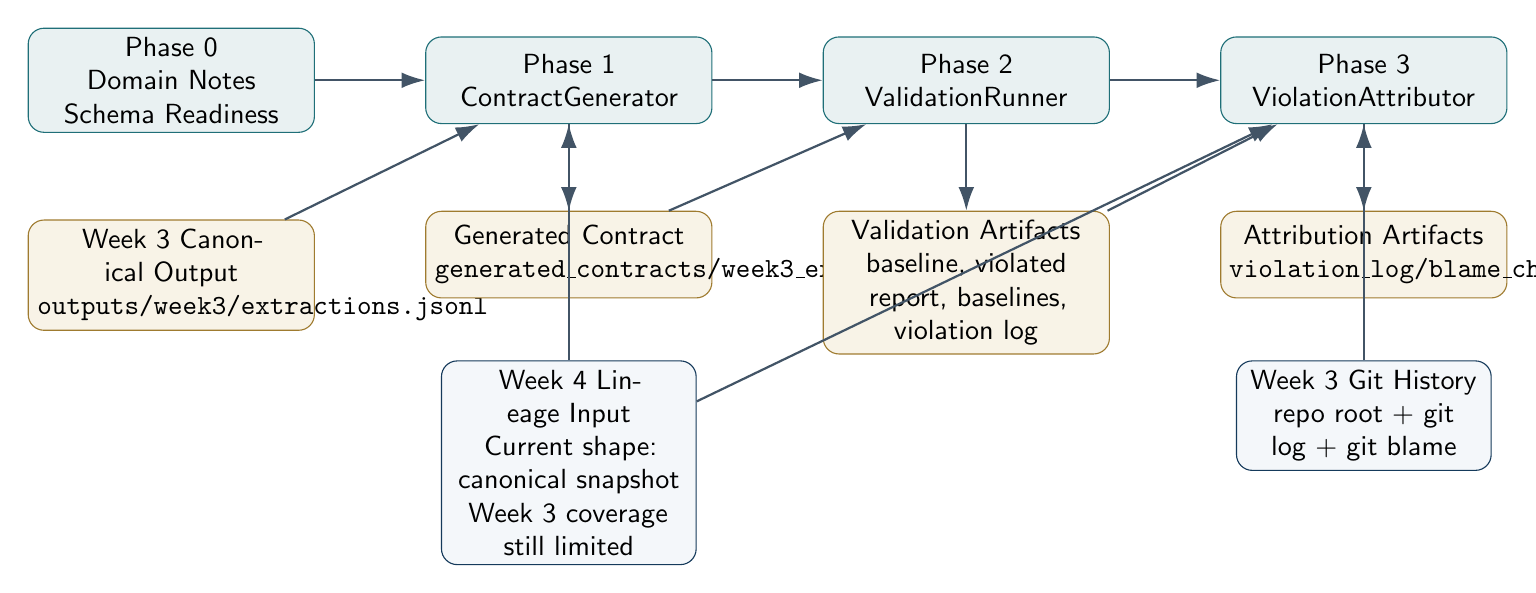
\begin{tikzpicture}[
  font=\sffamily,
  node distance=1.1cm and 1.4cm,
  box/.style={draw=navy, rounded corners=2mm, fill=mist, minimum width=3.0cm, minimum height=1.2cm, align=center, text width=3.0cm},
  phase/.style={draw=teal, rounded corners=2mm, fill=teal!10, minimum width=3.4cm, minimum height=1.1cm, align=center, text width=3.4cm},
  artifact/.style={draw=gold!80!black, rounded corners=2mm, fill=gold!12, minimum width=3.4cm, minimum height=1.1cm, align=center, text width=3.4cm},
  arrow/.style={-{Latex[length=3mm,width=2mm]}, thick, draw=slate}
]
  \node[phase] (phase0) {Phase 0\\Domain Notes\\Schema Readiness};
  \node[phase, right=of phase0] (phase1) {Phase 1\\ContractGenerator};
  \node[phase, right=of phase1] (phase2) {Phase 2\\ValidationRunner};
  \node[phase, right=of phase2] (phase3) {Phase 3\\ViolationAttributor};

  \node[artifact, below=1.1cm of phase0] (week3) {Week 3 Canonical Output\\\texttt{outputs/week3/extractions.jsonl}};
  \node[artifact, below=1.1cm of phase1] (contract) {Generated Contract\\\texttt{generated\_contracts/week3\_extractions.yaml}};
  \node[artifact, below=1.1cm of phase2] (reports) {Validation Artifacts\\baseline, violated report, baselines, violation log};
  \node[artifact, below=1.1cm of phase3] (blame) {Attribution Artifacts\\\texttt{violation\_log/blame\_chain.json}};

  \node[box, below=3.0cm of phase1] (lineage) {Week 4 Lineage Input\\Current shape: canonical snapshot\\Week 3 coverage still limited};
  \node[box, below=3.0cm of phase3] (git) {Week 3 Git History\\repo root + git log + git blame};

  \draw[arrow] (phase0) -- (phase1);
  \draw[arrow] (phase1) -- (phase2);
  \draw[arrow] (phase2) -- (phase3);

  \draw[arrow] (week3) -- (phase1);
  \draw[arrow] (phase1) -- (contract);
  \draw[arrow] (contract) -- (phase2);
  \draw[arrow] (phase2) -- (reports);
  \draw[arrow] (reports) -- (phase3);
  \draw[arrow] (phase3) -- (blame);

  \draw[arrow] (lineage) -- (phase1);
  \draw[arrow] (lineage) -- (phase3);
  \draw[arrow] (git) -- (phase3);
\end{tikzpicture}
}
\caption{Architecture through Phase 3.}
\end{figure}

\section{Architectural interpretation}
This architecture has one strong center of gravity: Week 3 canonical extractions. Everything implemented so far either describes that interface, validates it, or attributes failures against it.

\begin{itemize}[leftmargin=1.5em]
  \item \textbf{Phase 0} established whether the upstream outputs were usable and where canonicalization was necessary.
  \item \textbf{Phase 1} turned the real Week 3 payload into a human-readable contract with structural and numeric expectations.
  \item \textbf{Phase 2} operationalized that contract by running it on clean and violated snapshots.
  \item \textbf{Phase 3} converted a validation failure into an engineering triage path using git-backed attribution.
\end{itemize}

\section{Design strengths}
\begin{itemize}[leftmargin=1.5em]
  \item The pipeline is \textbf{evidence-first}. Contracts are inferred from real data, not predefined in isolation.
  \item The validator is \textbf{semantic-aware}. It detects confidence scale drift that would pass a naive type check.
  \item Attribution is \textbf{explainable}. It uses path relevance, line-level blame, and recent git history rather than opaque heuristics.
\end{itemize}

\section{Architectural weakness that still matters}
The weakest part of the architecture is not the validator or the blame logic. It is the current Week 4 lineage input. Because the lineage file is not modeling the Week 3 extraction system directly, blast radius remains conservative and low-confidence.

\clearpage
\chapter{Phase 0 -- Domain Analysis and Readiness}

\section{What Phase 0 proved}
Phase 0 established that the Week 7 project could not be built responsibly on top of raw upstream files without understanding where they diverged from canonical expectations. The outcome was a stronger \texttt{DOMAIN\_NOTES.md} and a clear migration-first path instead of jumping straight into code generation.

\section{Most important Phase 0 findings}
\begin{itemize}[leftmargin=1.5em]
  \item Week 1 and Week 2 were usable as evidence but not the main contract target.
  \item Week 3 originally lacked the canonical nested extraction shape needed for fact-level contract checks.
  \item Week 4 existed at the expected path and was later migrated into the canonical Week 7 snapshot interface, though the current snapshots still do not expose an explicit Week 3 consumer path.
  \item Week 5 had sufficient volume but needed an event-envelope migration to fully align with canonical expectations.
  \item LangSmith traces were present and useful, but trace normalization remains a later concern.
\end{itemize}

\section{Why this mattered for the implementation}
Without this Phase 0 work, the rest of the implementation would have been misleading. The ContractGenerator would have described the wrong Week 3 shape, the validator would have checked the wrong field, and the attribution story would have looked more precise than the data justified.

\section{Readiness result}
Phase 0 succeeded because it forced the implementation to be grounded in the actual interfaces that now exist in the repository. That is why later phases were able to use \texttt{fact\_confidence} rather than a legacy summary field.

\clearpage
\chapter{Phase 1 -- ContractGenerator Design and Output}

\section{Design goal}
The ContractGenerator had to turn a real nested Week 3 extraction dataset into a readable Bitol-style YAML contract that a human reviewer could inspect without needing to reverse-engineer raw JSON.

\section{Profiling strategy}
The central technical choice in Phase 1 was to flatten the dataset at the fact level rather than the document level. This was the correct choice because confidence is attached to extracted facts, not only to documents.

\begin{statusbox}{success}
\textbf{Key Phase 1 decision:} explode \texttt{extracted\_facts[]} into one profiled row per fact, while preserving document-level context such as \texttt{doc\_id}, source metadata, token counts, and runtime.
\end{statusbox}

\section{Field profiling results}
The generator now computes:
\begin{itemize}[leftmargin=1.5em]
  \item logical dtype
  \item null fraction
  \item cardinality estimate
  \item sample values
  \item numeric statistics for all numeric fields
\end{itemize}

The most important real result for this checkpoint is the observed confidence profile:

\begin{center}
\begin{tabular}{lrrr}
\toprule
Metric & Minimum & Maximum & Mean \\
\midrule
\texttt{fact\_confidence} & 0.55 & 1.00 & 0.80636 \\
\bottomrule
\end{tabular}
\end{center}

\section{Generated contract quality}
The resulting contract:
\begin{itemize}[leftmargin=1.5em]
  \item marks required fields clearly,
  \item enforces UUID and date-time formats where justified,
  \item constrains \texttt{fact\_confidence} to \texttt{0.0--1.0},
  \item preserves real observed statistics inside the profile blocks,
  \item injects lineage notes without fabricating downstream consumers.
\end{itemize}

\section{Phase 1 limitation}
The contract is good, but the lineage section is still weaker than it should be because Week 4 does not yet provide a canonical snapshot for the Week 3 system. This is a structural repository issue, not a Phase 1 logic error.

\clearpage
\chapter{Phase 2 -- ValidationRunner and Violation Testing}

\section{Validation strategy}
The ValidationRunner was designed to prove two things:

\begin{enumerate}[leftmargin=1.6em]
  \item a real Week 3 snapshot can pass a full validation run cleanly;
  \item a semantically dangerous but numerically valid confidence-scale change will still be caught.
\end{enumerate}

\section{Operational flow}
\begin{figure}[H]
\centering
\resizebox{0.93\textwidth}{!}{
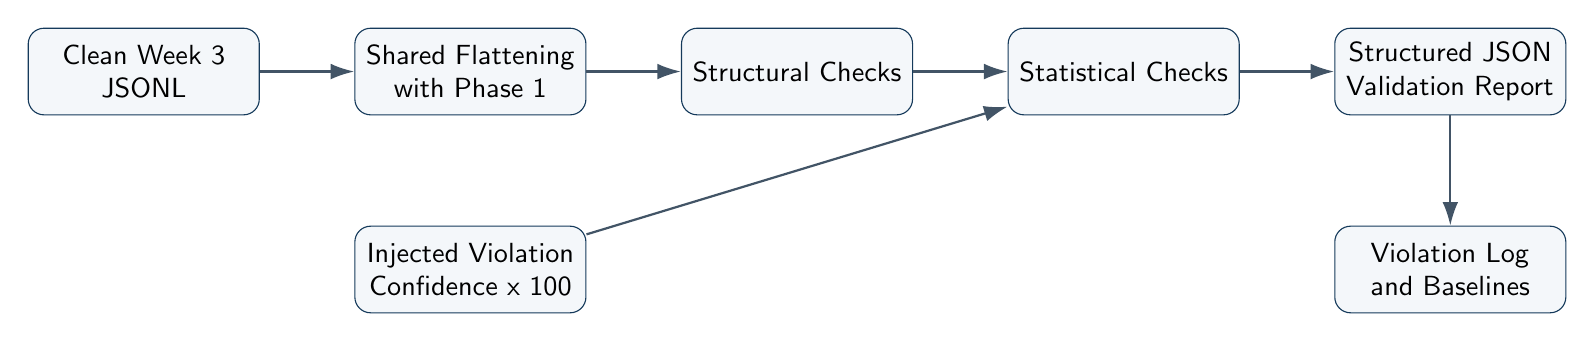
\begin{tikzpicture}[
  font=\sffamily,
  node distance=1.0cm and 1.2cm,
  box/.style={draw=navy, rounded corners=2mm, fill=mist, minimum width=2.7cm, minimum height=1.1cm, align=center, text width=2.7cm},
  arrow/.style={-{Latex[length=3mm,width=2mm]}, thick, draw=slate}
]
  \node[box] (clean) {Clean Week 3\\JSONL};
  \node[box, right=of clean] (flatten) {Shared Flattening\\with Phase 1};
  \node[box, right=of flatten] (struct) {Structural Checks};
  \node[box, right=of struct] (stats) {Statistical Checks};
  \node[box, right=of stats] (report) {Structured JSON\\Validation Report};

  \node[box, below=1.4cm of flatten] (violation) {Injected Violation\\Confidence x 100};
  \node[box, below=1.4cm of report] (log) {Violation Log\\and Baselines};

  \draw[arrow] (clean) -- (flatten);
  \draw[arrow] (flatten) -- (struct);
  \draw[arrow] (struct) -- (stats);
  \draw[arrow] (stats) -- (report);
  \draw[arrow] (violation) -- (stats);
  \draw[arrow] (report) -- (log);
\end{tikzpicture}
}
\caption{ValidationRunner flow used in the current implementation.}
\end{figure}

\section{Observed results}
\begin{center}
\renewcommand{\arraystretch}{1.2}
\begin{tabular}{lrrrr}
\toprule
Run & Total checks & Passed & Failed & Errored \\
\midrule
Clean rerun & 37 & 37 & 0 & 0 \\
Injected violation & 37 & 35 & 2 & 0 \\
\bottomrule
\end{tabular}
\end{center}

\section{Why the violation test is convincing}
The injected test is strong because it changes only the semantic scale of confidence. The field remains numeric, so the type system alone cannot save the pipeline. The validator catches the problem through:

\begin{itemize}[leftmargin=1.5em]
  \item a hard range failure on \texttt{fact\_confidence}; and
  \item a severe drift failure against the stored baseline.
\end{itemize}

\section{Important operational nuance}
Because the baseline file already existed on rerun, the clean report includes drift checks as well. This is expected behavior. It means the clean rerun now shows 37 checks instead of the 30 checks seen on the very first baseline build.

\section{Validation run evidence and interpretation}
The validation story is strongest when the report names the artifacts, states what they prove, and explains how to interpret them rather than simply listing pass/fail counts.

\begin{center}
\small
\setlength{\tabcolsep}{4pt}
\renewcommand{\arraystretch}{1.2}
\begin{tabularx}{\textwidth}{L{1.55in} L{1.65in} Y}
\toprule
Artifact & What it contains & Interpretation used in this report \\
\midrule
\codecell{validation_reports/thursday_baseline.json} & clean run against the canonical Week 3 snapshot & proves the contract is not over-constrained and that a real dataset can pass all active checks \\
\codecell{validation_reports/injected_violation.json} & failed run after multiplying fact confidence by 100 & proves the validator catches a semantic scale break that would survive a naive numeric type check \\
\codecell{violation_log/violations.jsonl} & structured non-pass findings across runs & proves failures are logged in machine-readable form suitable for later attribution and report generation \\
\codecell{schema_snapshots/baselines.json} & stored numeric baselines for drift checks & proves drift detection is grounded in measured prior behavior rather than arbitrary thresholds \\
\bottomrule
\end{tabularx}
\end{center}

The interpretation of the two failed checks matters:

\begin{itemize}[leftmargin=1.5em]
  \item \textbf{Range failure} means the contract has a precise boundary and the violated snapshot crossed it directly.
  \item \textbf{Drift failure} means the data also became statistically implausible compared to the baseline, which is exactly the behavior Week 7 is supposed to surface before silent downstream corruption.
  \item \textbf{Zero execution errors} on both runs means the validation framework itself stayed stable under both clean and bad input.
\end{itemize}

\clearpage
\chapter{Phase 3 -- ViolationAttributor and Blame Chain}

\section{Design goal}
The goal of Phase 3 was not to produce a perfect forensic truth engine. The goal was to convert a failed validation result into a plausible, explainable blame chain that an engineer could use as a starting point for debugging and remediation.

\section{Attribution flow}
\begin{figure}[H]
\centering
\resizebox{\textwidth}{!}{
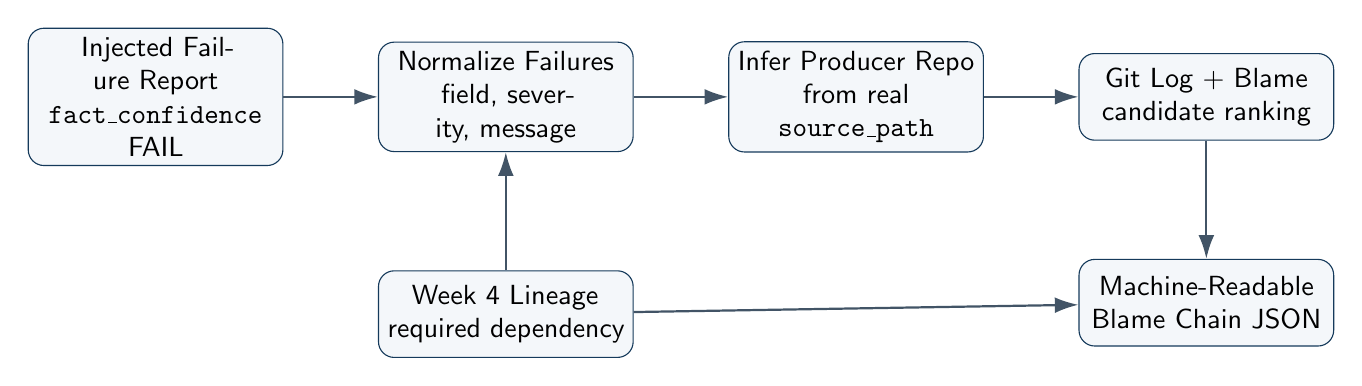
\begin{tikzpicture}[
  font=\sffamily,
  node distance=1.1cm and 1.2cm,
  box/.style={draw=navy, rounded corners=2mm, fill=mist, minimum width=3.0cm, minimum height=1.1cm, align=center, text width=3.0cm},
  arrow/.style={-{Latex[length=3mm,width=2mm]}, thick, draw=slate}
]
  \node[box] (fail) {Injected Failure Report\\\texttt{fact\_confidence} FAIL};
  \node[box, right=of fail] (normalize) {Normalize Failures\\field, severity, message};
  \node[box, right=of normalize] (repo) {Infer Producer Repo\\from real \texttt{source\_path}};
  \node[box, right=of repo] (git) {Git Log + Blame\\candidate ranking};

  \node[box, below=1.5cm of normalize] (lineage) {Week 4 Lineage\\required dependency};
  \node[box, below=1.5cm of git] (output) {Machine-Readable\\Blame Chain JSON};

  \draw[arrow] (fail) -- (normalize);
  \draw[arrow] (normalize) -- (repo);
  \draw[arrow] (repo) -- (git);
  \draw[arrow] (git) -- (output);
  \draw[arrow] (lineage) -- (normalize);
  \draw[arrow] (lineage) -- (output);
\end{tikzpicture}
}
\caption{ViolationAttributor flow used in the current implementation.}
\end{figure}

\section{Top attribution result}
The strongest blame-chain candidate for both injected failures is:

\begin{callout}
\textbf{Top producer-side file:} \texttt{src/agents/fact\_table.py}\\
\textbf{Top commit:} \texttt{033135cc46c7b8889cb8bf4f6607f940469bed5b}\\
\textbf{Author:} Birkity \texttt{<birkity.yishak.m@gmail.com>}\\
\textbf{Why it matters:} this file assigns and persists fact-level confidence values and therefore sits on the most direct path between extraction logic and the failing contract field.
\end{callout}

\section{Why this result is defensible}
This attribution is not just based on file names. It is supported by:

\begin{itemize}[leftmargin=1.5em]
  \item token-level relevance to the failing field,
  \item line-level blame on the confidence assignment block,
  \item recent commit history on the same file,
  \item corroboration from the Week 3 schema file and strategy files.
\end{itemize}

\section{What blast radius currently means}
The current blast radius is intentionally conservative because the Week 4 lineage graph does not expose real Week 3 consumers. The correct interpretation is:

\begin{itemize}[leftmargin=1.5em]
  \item producer attribution is strong;
  \item downstream dependency mapping is weak;
  \item the system reports that weakness explicitly instead of inventing false certainty.
\end{itemize}

\clearpage
\chapter{Artifact Inventory and Deliverables}

\section{Core implementation artifacts}
{\small
\setlength{\tabcolsep}{4pt}
\begin{longtable}{L{1.45in} L{1.95in} L{2.45in}}
\toprule
Artifact & Location & Purpose \\
\midrule
\endfirsthead
\toprule
Artifact & Location & Purpose \\
\midrule
\endhead
Domain notes & \codecell{DOMAIN_NOTES.md} & Phase 0 reasoning and system-specific failure analysis \\
Phase 0 report & \codecell{reports/phase_0.md} & readiness and migration findings \\
ContractGenerator & \codecell{contracts/generator.py} & profiles real Week 3 data and generates YAML contract \\
Week 3 contract & \codecell{generated_contracts/week3_extractions.yaml} & machine-readable contract for Week 3 interface \\
Week 3 dbt counterpart & \codecell{generated_contracts/week3_extractions_dbt.yml} & dbt-compatible test translation of the Week 3 contract \\
Week 5 contract & \codecell{generated_contracts/week5_events.yaml} & machine-readable contract for the event-stream interface \\
Week 5 dbt counterpart & \codecell{generated_contracts/week5_events_dbt.yml} & dbt-compatible test translation of the Week 5 contract \\
Phase 1 report & \codecell{reports/phase_1.md} & methodology and profiling results \\
ValidationRunner & \codecell{contracts/runner.py} & structural and statistical validation engine \\
Baseline validation & \codecell{validation_reports/thursday_baseline.json} & clean validation evidence \\
Injected validation & \codecell{validation_reports/injected_violation.json} & violated snapshot evidence \\
Violation log & \codecell{violation_log/violations.jsonl} & structured non-pass findings \\
Baselines & \codecell{schema_snapshots/baselines.json} & numeric drift reference values \\
ViolationAttributor & \codecell{contracts/attributor.py} & git-backed blame chain generator \\
Blame chain output & \codecell{violation_log/blame_chain.json} & ranked attribution candidates and blast-radius summary \\
Phase 3 report & \codecell{reports/phase_3.md} & attribution logic, evidence, and limitations \\
\bottomrule
\end{longtable}
}

\section{Contract coverage table completeness and rationale}
The current contract inventory should be judged not only by the number of generated files, but by whether the coverage decisions are explainable. The table below states both the current coverage and the reason each interface is or is not fully covered at this checkpoint.

\begin{center}
\small
\setlength{\tabcolsep}{4pt}
\renewcommand{\arraystretch}{1.22}
\begin{tabularx}{\textwidth}{L{0.95in} L{1.55in} L{1.55in} Y}
\toprule
System & Bitol contract & dbt counterpart & Rationale \\
\midrule
Week 1 & not generated yet & not generated yet & usable evidence source in Phase 0, but not prioritized because Week 3 carried higher downstream risk and nested data complexity \\
Week 2 & not generated yet & not generated yet & useful for future envelope-level validation, but lower immediate risk than Week 3 confidence semantics \\
Week 3 & \codecell{week3_extractions.yaml} & \codecell{week3_extractions_dbt.yml} & fully prioritized because it is the main monitored interface and supports the injected confidence-scale test \\
Week 4 & not generated as contract & not generated as contract & current artifact is lineage input rather than a stabilized business dataset contract target; it is canonical now, but not the main contract target \\
Week 5 & \codecell{week5_events.yaml} & \codecell{week5_events_dbt.yml} & generated to strengthen multi-system coverage and satisfy the minimum deliverable expectation from the project spec \\
LangSmith traces & not generated yet & not applicable & present as supporting evidence for later AI-specific contract extensions rather than the current core path \\
\bottomrule
\end{tabularx}
\end{center}

This table is complete enough for review because it distinguishes between:

\begin{itemize}[leftmargin=1.5em]
  \item \textbf{covered and implemented} interfaces,
  \item \textbf{deliberately deferred} interfaces, and
  \item interfaces whose current upstream shape makes contract generation less honest or less useful.
\end{itemize}

\section{Implementation readiness}
\begin{statusbox}{success}
\textbf{Ready for implementation review:} yes.
\end{statusbox}

This is a fair claim because the repository now contains:
\begin{itemize}[leftmargin=1.5em]
  \item real data contracts,
  \item real validation outputs,
  \item a real injected violation and successful detection,
  \item a real blame-chain output based on a local git repository.
\end{itemize}

\section{Important caveat for reviewers}
The repository is stronger in contract, validation, and attribution logic than it is in lineage quality. Reviewers should judge the current weakness as an upstream input limitation, not a failure of the implemented Phase 1--3 code paths.

\clearpage
\chapter{Risks, Gaps, and Improvement Opportunities}

\section{Highest-risk technical gap}
The highest-risk unresolved gap is the Week 4 lineage snapshot. It is currently the limiting factor for attribution quality, blast radius completeness, and later report generation.

\section{Other meaningful gaps}
\begin{itemize}[leftmargin=1.5em]
  \item Week 1, Week 2, and LangSmith traces do not yet have generated contracts, so coverage is still concentrated on the highest-value interfaces rather than the entire platform.
  \item The violation log currently appends duplicate injected failures on rerun.
  \item The blame-chain output does not yet emit exact line ranges.
  \item Schema evolution and AI extension phases are not yet implemented.
\end{itemize}

\section{Best next steps}
\begin{enumerate}[leftmargin=1.6em]
  \item Expand Week 4 lineage coverage so the canonical snapshots expose an explicit Week 3 consumer path.
  \item Expand contract generation to Week 1, Week 2, and selected trace interfaces.
  \item Build SchemaEvolutionAnalyzer on top of stored contract snapshots.
  \item Add AI Contract Extensions for trace and embedding-aware checks.
  \item Generate the final Enforcer Report from live artifacts rather than writing summary prose by hand.
\end{enumerate}

\section{What would strengthen the final submission}
The final submission would be stronger if it showed:

\begin{itemize}[leftmargin=1.5em]
  \item two or more real contracts generated from different systems,
  \item one real violation in addition to the injected violation,
  \item a canonical Week 4 lineage graph that yields non-empty blast radius,
  \item a machine-generated final report understandable by a non-engineer.
\end{itemize}

\section{Reflection quality and learning depth}
The most important learning from this build is that contract systems are only as trustworthy as their upstream realism. The repository improved substantially when the team stopped trying to force Phase 1 and Phase 2 onto legacy Week 3 shapes and instead migrated the data into the canonical interface first. That changed the work from a synthetic demo into an evidence-based implementation.

A second lesson is that structural validation alone is not enough. The confidence violation is a good test precisely because nothing about the field's type looks obviously broken after the scale change. The current implementation therefore reinforced a practical engineering truth: a validator that only checks names and dtypes can still allow severe business corruption to pass through cleanly.

The third lesson is about humility in attribution. The current Phase 3 output is strongest where the data is strongest: producer-side git evidence. It is weaker where the lineage input is weaker: downstream blast radius. Writing that limitation explicitly made the report better, not worse, because it shows that the system distinguishes between measured certainty and unsupported guesswork.

Overall, the implementation deepened one central understanding: the real value of a contract-enforcement platform is not just rejecting bad data. It is making system boundaries legible, measurable, and explainable enough that a team can act quickly when change happens.

\clearpage
\chapter{Conclusion}

This report demonstrates a working contract-enforcement pipeline through Phase 3. The implementation is grounded in real repository artifacts, real Week 3 data, real validation runs, and real source-side git history. The strongest proof point is not that the validator can fail a bad file. The strongest proof point is that the system can trace that failure back to the most likely producer-side file and commit while also stating, plainly, where its certainty ends.

\begin{callout}
\textbf{Final verdict}

The current implementation is technically credible and operational through Phase 3. The repository is not yet the full Week 7 system, but it already demonstrates the core engineering behavior that the final system must preserve: contract generation from real data, semantic validation against live distributions, and explainable attribution of detected failures.
\end{callout}

\vfill
\begin{center}
{\large\bfseries\color{navy} Birkity Yishak}\\
\textcolor{slate}{TRP Week 7 Challenge -- Data Contract Enforcer}
\end{center}

\end{document}
